\chapter{Continued Pretraining on TabPFN}
\label{chap:continuedpretraining}
This chapter will focus on our third and final method for training and, presumably, improving the performance of TabPFN-TS on the GIFT-Eval dataset: continued pretraining.
Instead of using real-world data, as in the methods of the previous chapter, we now generate artificial time series to train TabPFN-TS.
\section{Experimental Setup}
The experimental setup is similar to the one we used to finetune TabPFN with real-world datasets, as we mostly use the same code.
The key differences for the current procedure are in data loading, validation, and hyperparameters.
\subsubsection{Data loading}
As mentioned above, instead of taking data from real-world datasets as we did in the methods before, we now sample artificial time series.
This is done with the code provided by \citep{dooley2023forecastpfn} that generates these time series based on a given context length(that represents the length of the time series) and frequency (that later determines the prediction length of the time series).
This was further explained in %TODO hier ref zu background
To train TabPFN with a broad mass of artificial time series data, we also have to sample from a wide range of context lengths as well as frequencies.
For this, we firstly specify a set of context lengths and frequencies that the prior will use to generate data from.
After that, in every epoch, the dataloader samples a context length as well as a frequency and generates enough time series with these parameters to create a batch.

The context lengths we will be using are
\[32,\space 64,\space 96,\space 128,\space 192,\space 256,\space 384,\space 512,\space 768,\space 1024,\space 2048,\space 4096\]
And the frequencies we will sample from are
\[hourly, daily, weekly, monthly, yearly\]
\subsubsection{Validation}
Validation is done similarly to what we did with multi-dataset finetuning.
As a prior only generates artificial data, it is not possible to validate the current state of the model on it, and this would lead to ...
Since we later apply TabPFN only to real-world datasets, we also need to validate it on them.
For this endeavor, we selected a subset of the datasets currently in GIFT-Eval that provide a wide range of different metadata.
This includes context length, frequency, and other special features that are not easy to quantify but can be seen, e.g., \ noisiness.

For validation datasets, we chose:
\begin{table}[h]
\centering
\begin{tabular}{lccc}
\hline
Dataset & Context Length & Frequency & \# Time Series \\
\hline
SZ\_TAXI/H & 744 & H & 156 \\
electricity/H & 4096 & H & 370 \\
electricity/W & 208 & W & 370 \\
LOOP\_SEATTLE/D & 365 & D & 323 \\
solar/W & 52 & W & 137 \\
us\_births/D & 4096 & D & 1 \\
M\_DENSE/D & 730 & D & 30 \\
covid\_deaths & 212 & D & 266 \\
SZ\_TAXI/15T & 2976 & 15T & 156 \\
hierarchical\_sales/D & 1825 & D & 118 \\
hierarchical\_sales/W & 260 & W & 118 \\
saugeenday/W & 3391 & W & 1 \\
\hline
\end{tabular}
\caption{}
\end{table}
\subsubsection{Hyperparameters}
Different from our finetuning setup, we do not take the batch sizes 16, 32, and 64 into account.
In an earlier test run, these batch sizes showed little to no training progress, as batch generation took too long due to the creation of time series.
\newline
The second setting that is different is the time limit.
Instead of training for a maximum time of 2400 seconds or 40 minutes, with continued pretraining, we train for 3600 seconds or 60 minutes.
This is also due to the fact that dynamically generating time series takes longer than using real-world data.
\section{Results}
After evaluating the top 5 checkpoints we selected based on their best validation loss on the datasets mentioned above, we have now accumulated the following results.
\begin{figure}[H]
    \centering

    \begin{subfigure}[t]{0.3\textwidth}
        \centering
        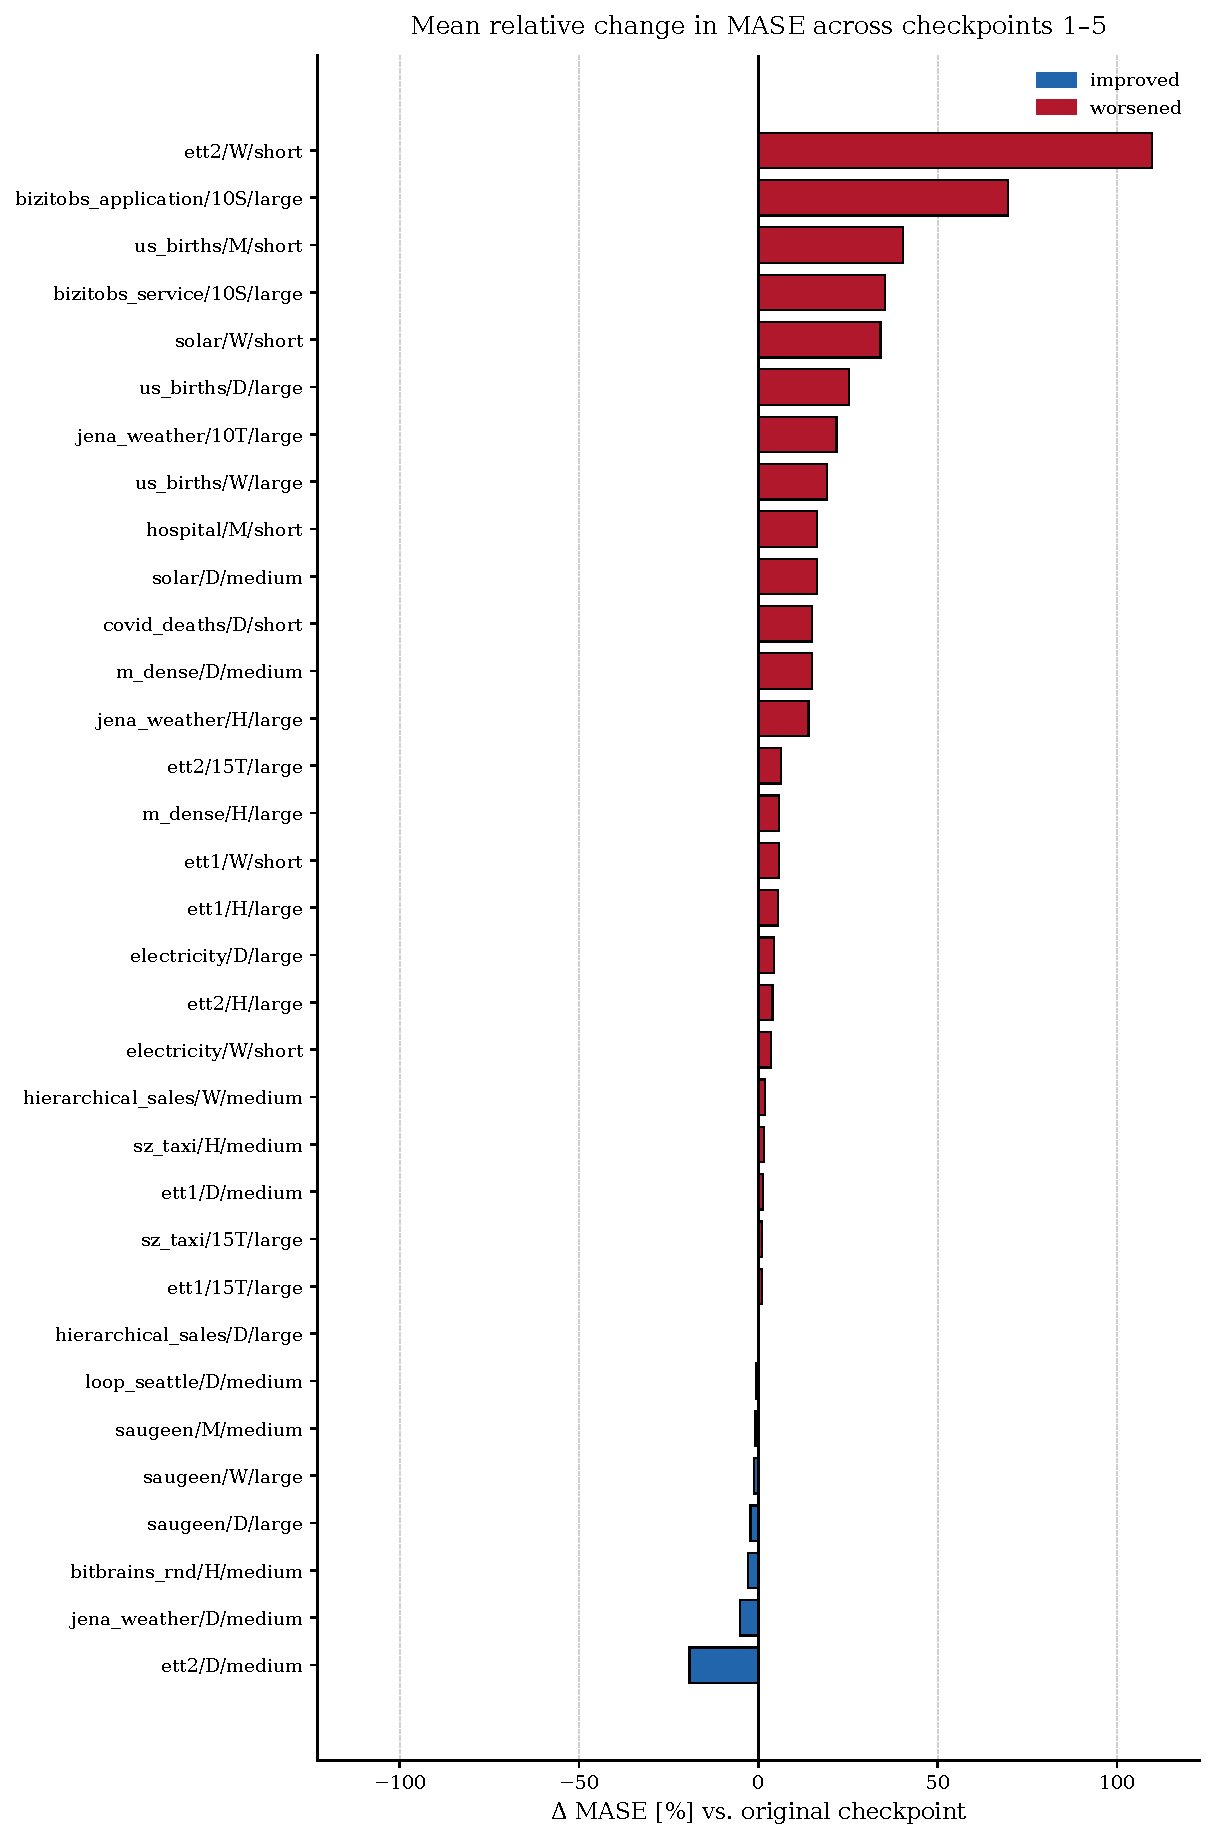
\includegraphics[width=\linewidth]{pictures/prior/mase_mean_delta_plot.pdf}
        \caption{Mean delta over all checkpoints}
        \label{fig:mase_mean_delta_plot}
    \end{subfigure}
    \hfill
    \begin{subfigure}[t]{0.3\textwidth}
        \centering
        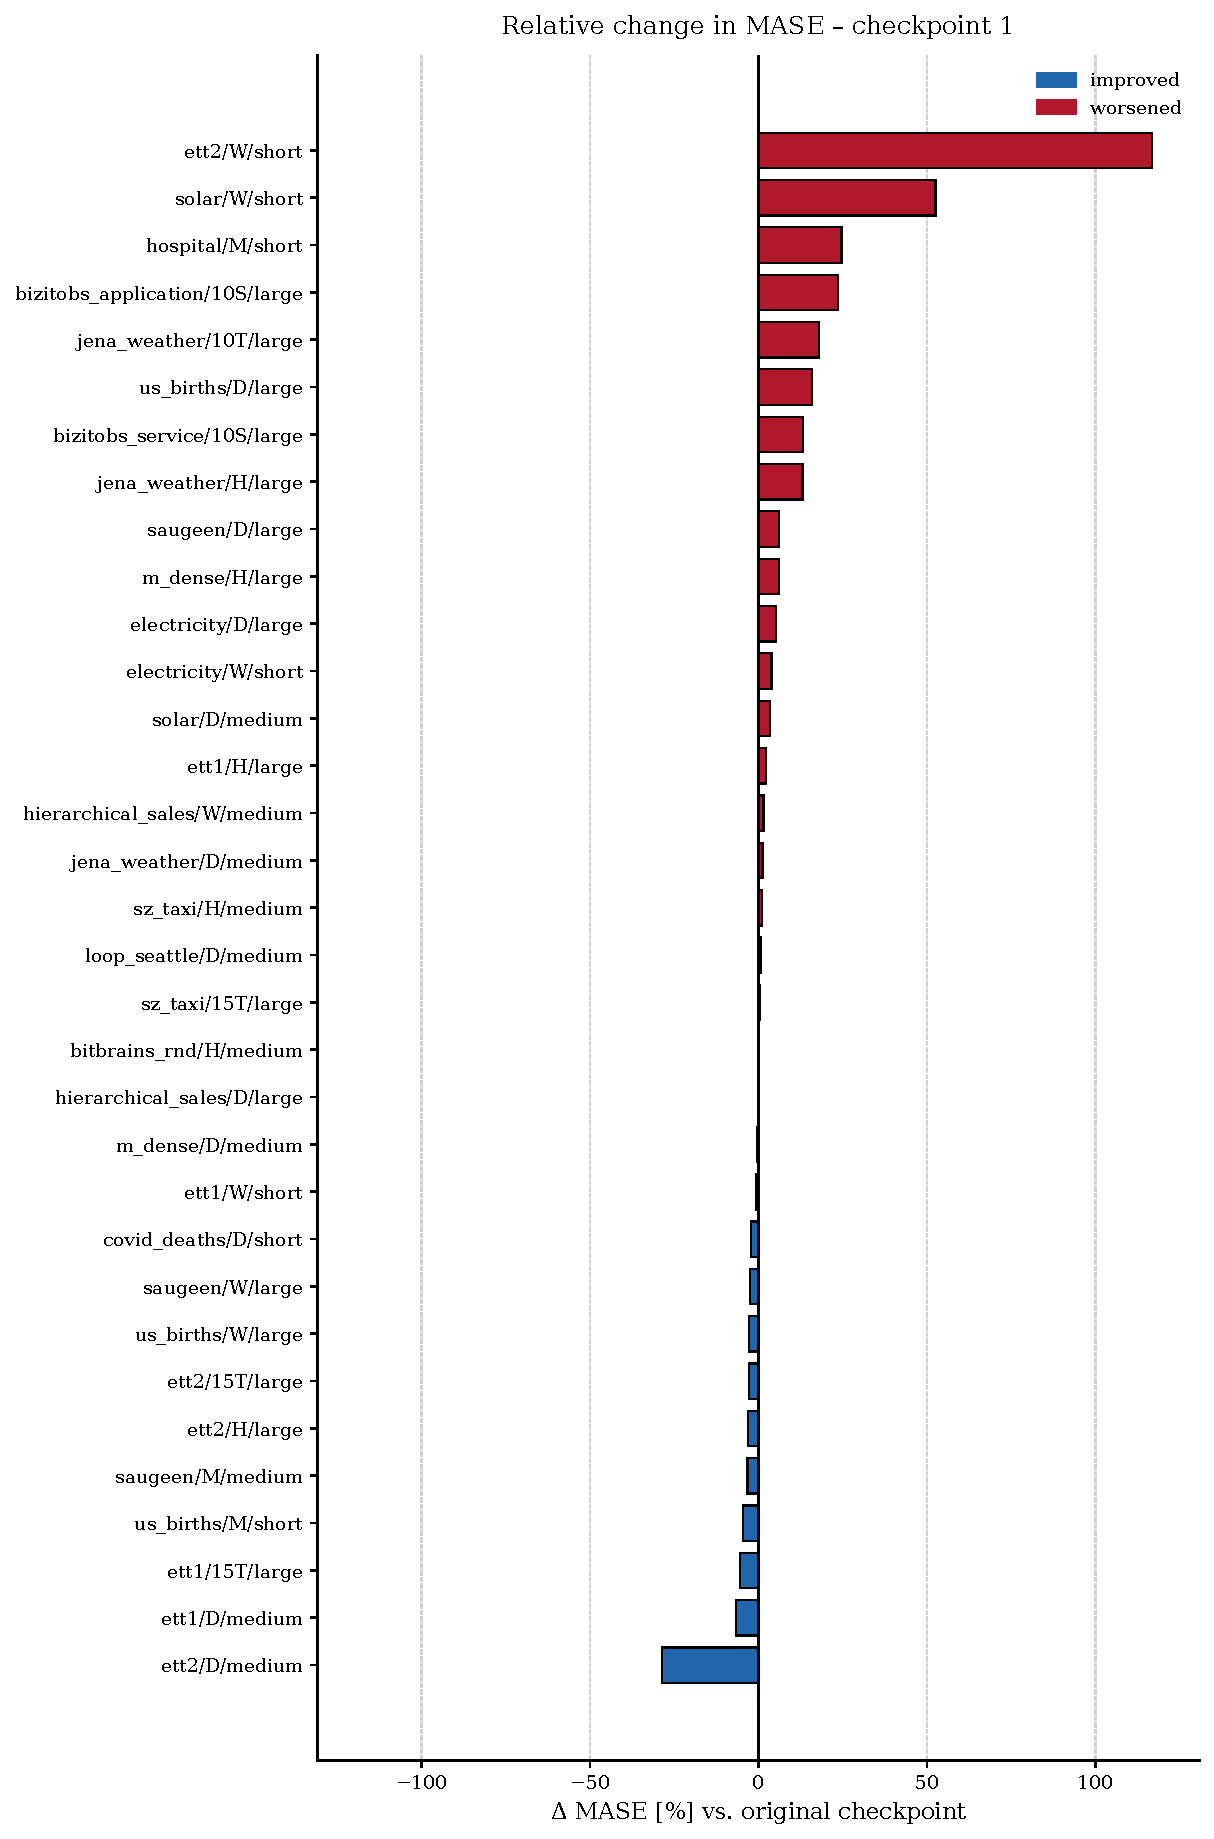
\includegraphics[width=\linewidth]{pictures/prior/mase_ckpt_1_delta_plot.pdf}
        \caption{Delta of checkpoint 1}
        \label{fig:mase_ckpt_1_delta_plot}
    \end{subfigure}
    \hfill
    \begin{subfigure}[t]{0.3\textwidth}
        \centering
        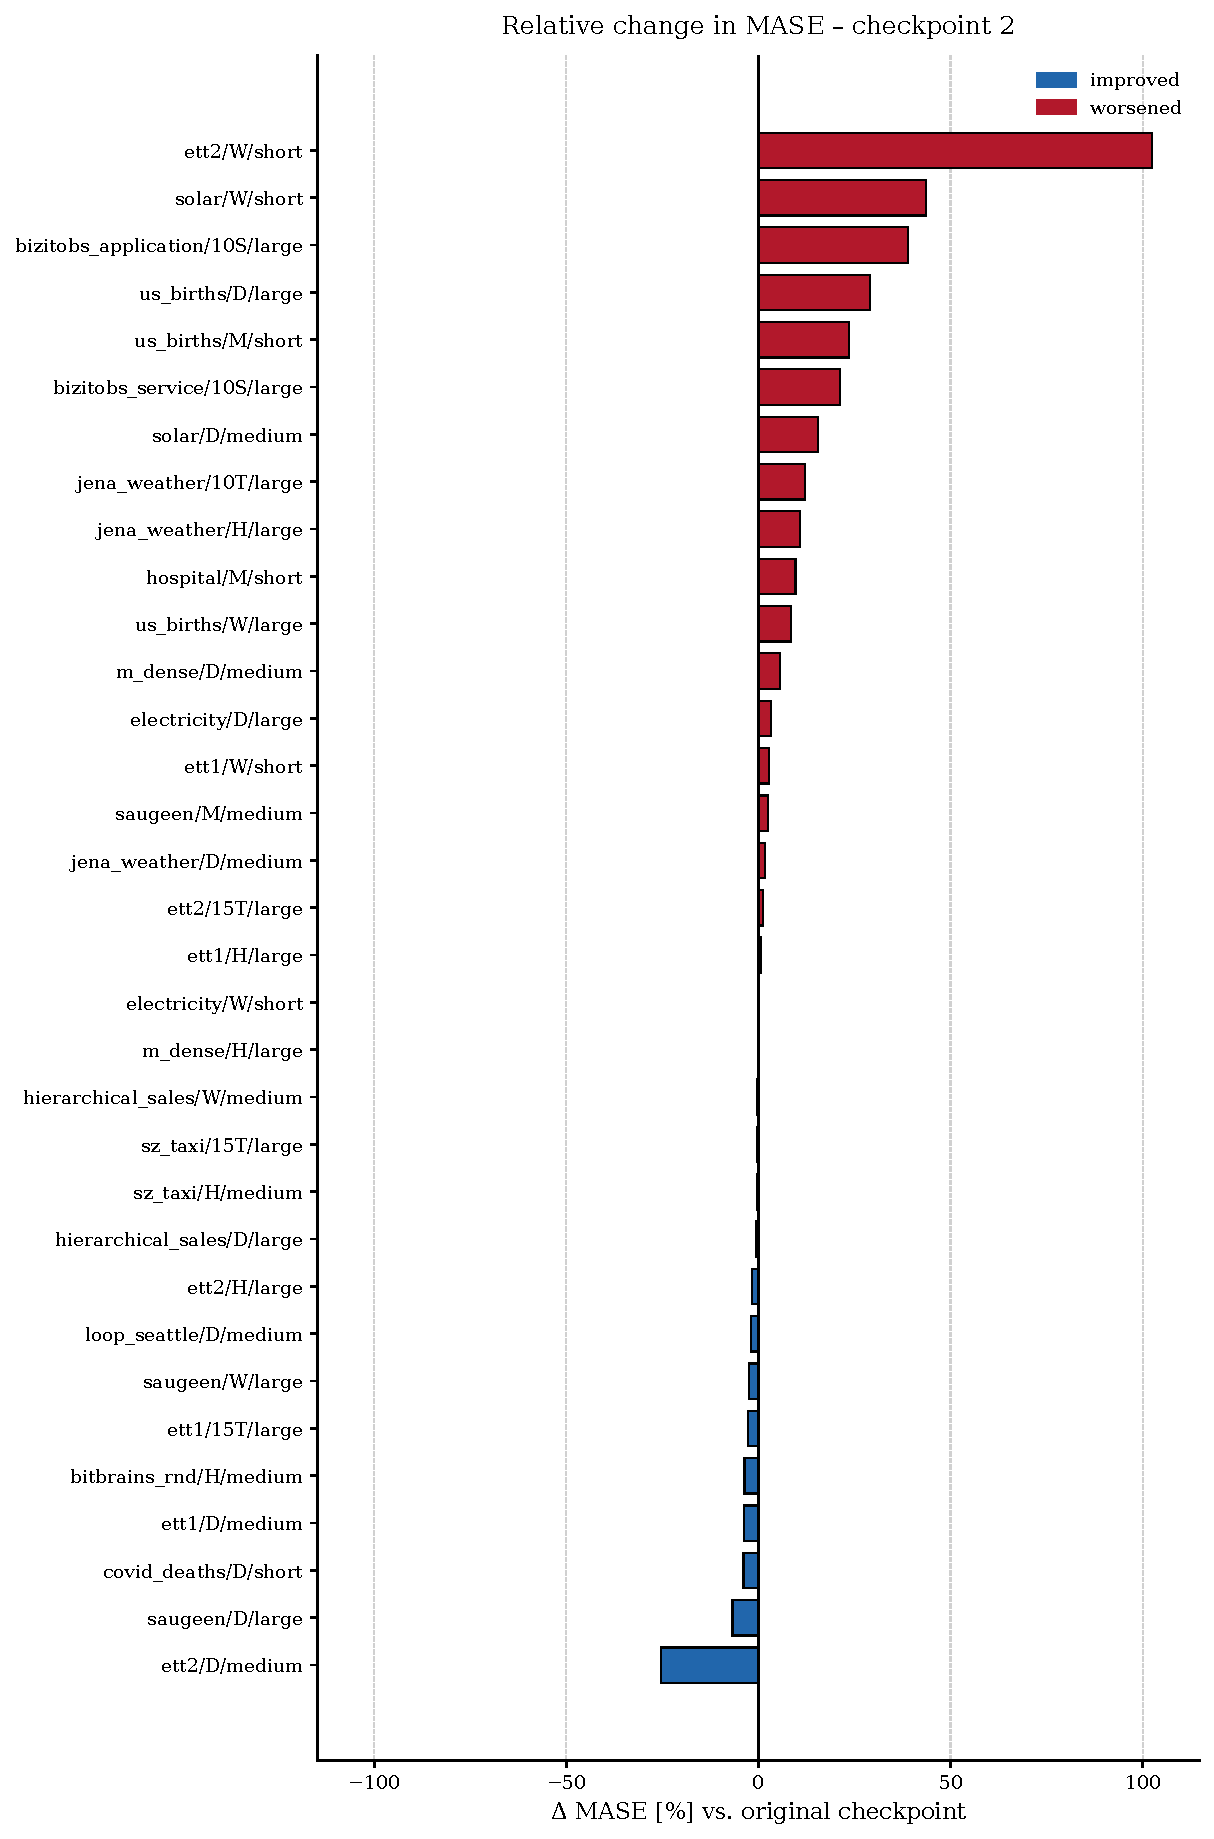
\includegraphics[width=\linewidth]{pictures/prior/mase_ckpt_2_delta_plot.pdf}
        \caption{Delta of checkpoint 2}
        \label{fig:mase_ckpt_2_delta_plot}
    \end{subfigure}

    \vspace{0.5cm}

    \begin{subfigure}[t]{0.3\textwidth}
        \centering
        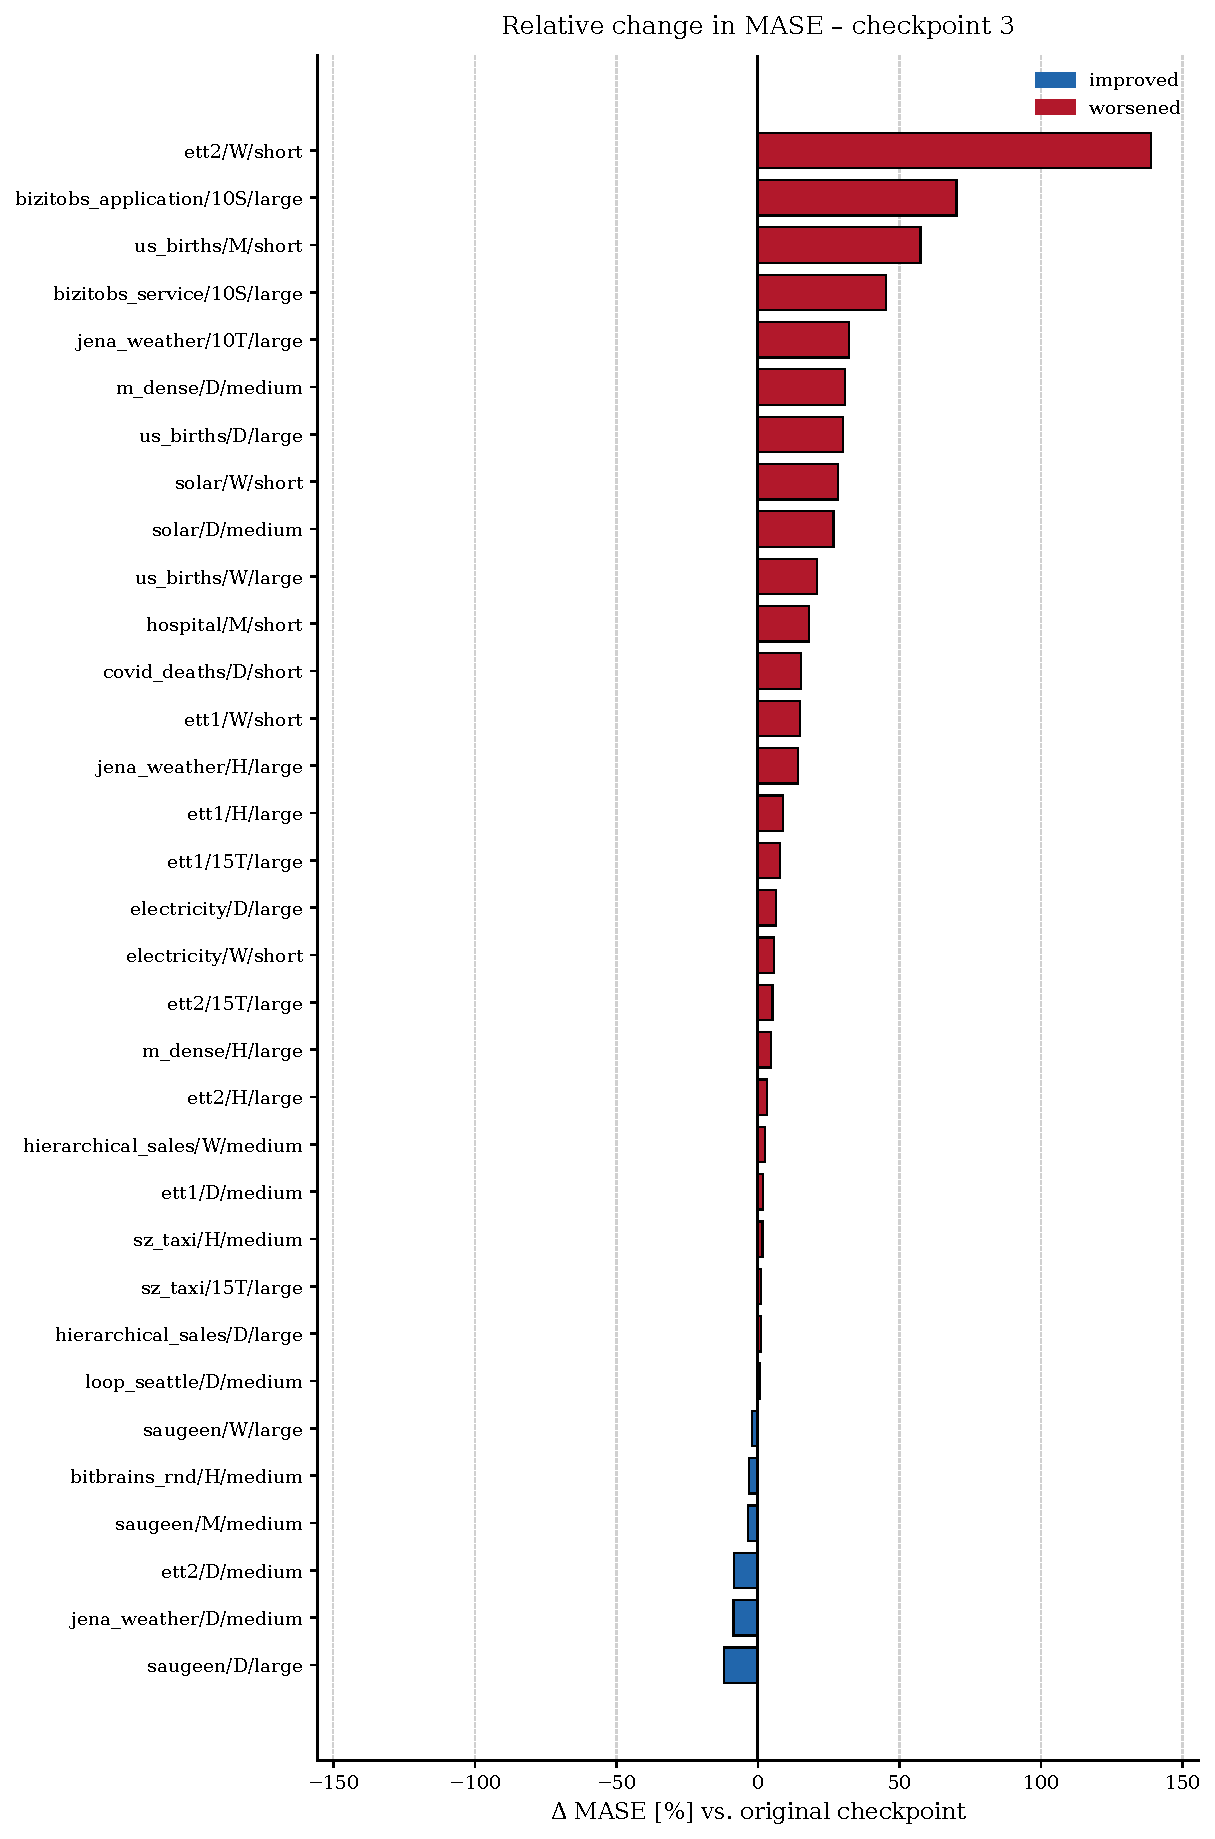
\includegraphics[width=\linewidth]{pictures/prior/mase_ckpt_3_delta_plot.pdf}
        \caption{Delta of checkpoint 3}
        \label{fig:mase_ckpt_3_delta_plot}
    \end{subfigure}
    \hfill
    \begin{subfigure}[t]{0.3\textwidth}
        \centering
        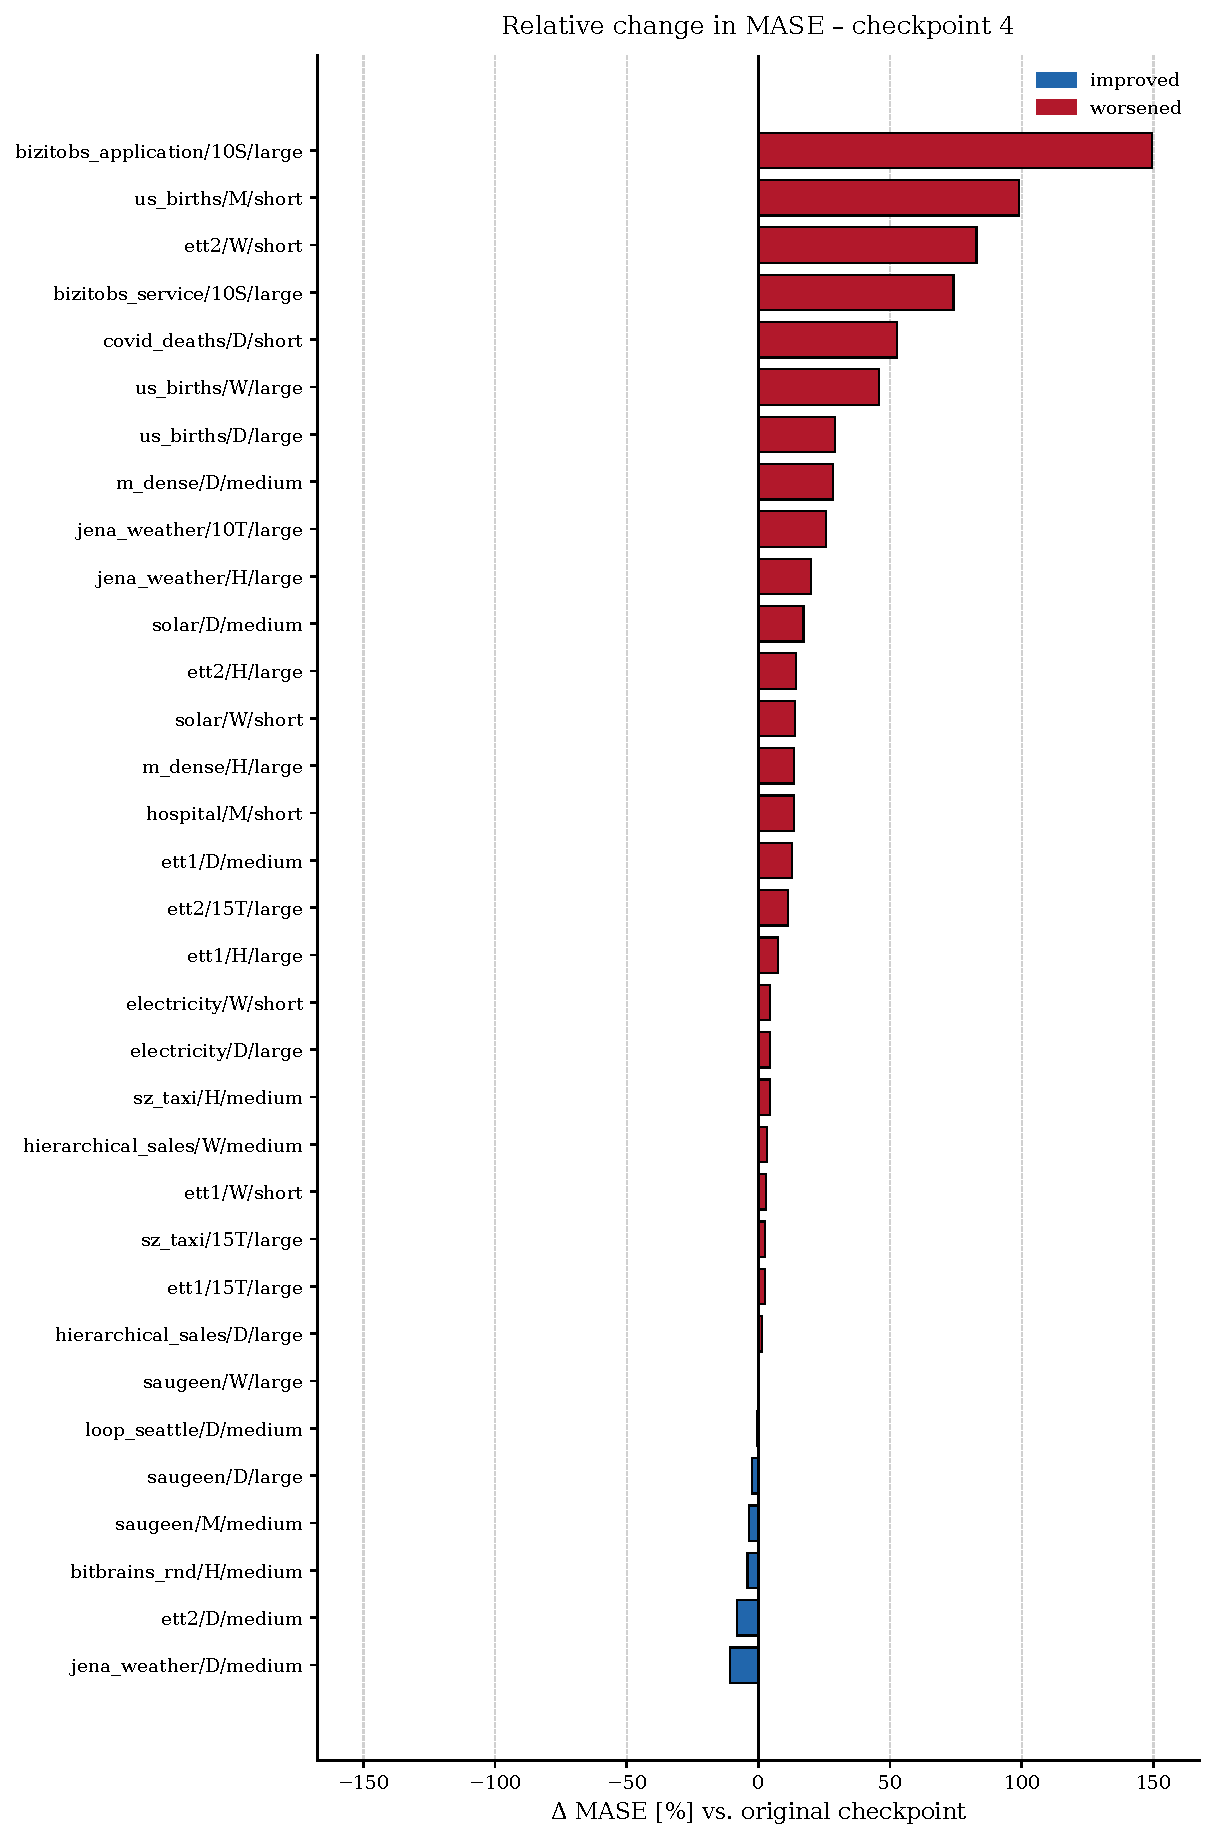
\includegraphics[width=\linewidth]{pictures/prior/mase_ckpt_4_delta_plot.pdf}
        \caption{Delta of checkpoint 4}
        \label{fig:mase_ckpt_4_delta_plot}
    \end{subfigure}
    \hfill
    \begin{subfigure}[t]{0.3\textwidth}
        \centering
        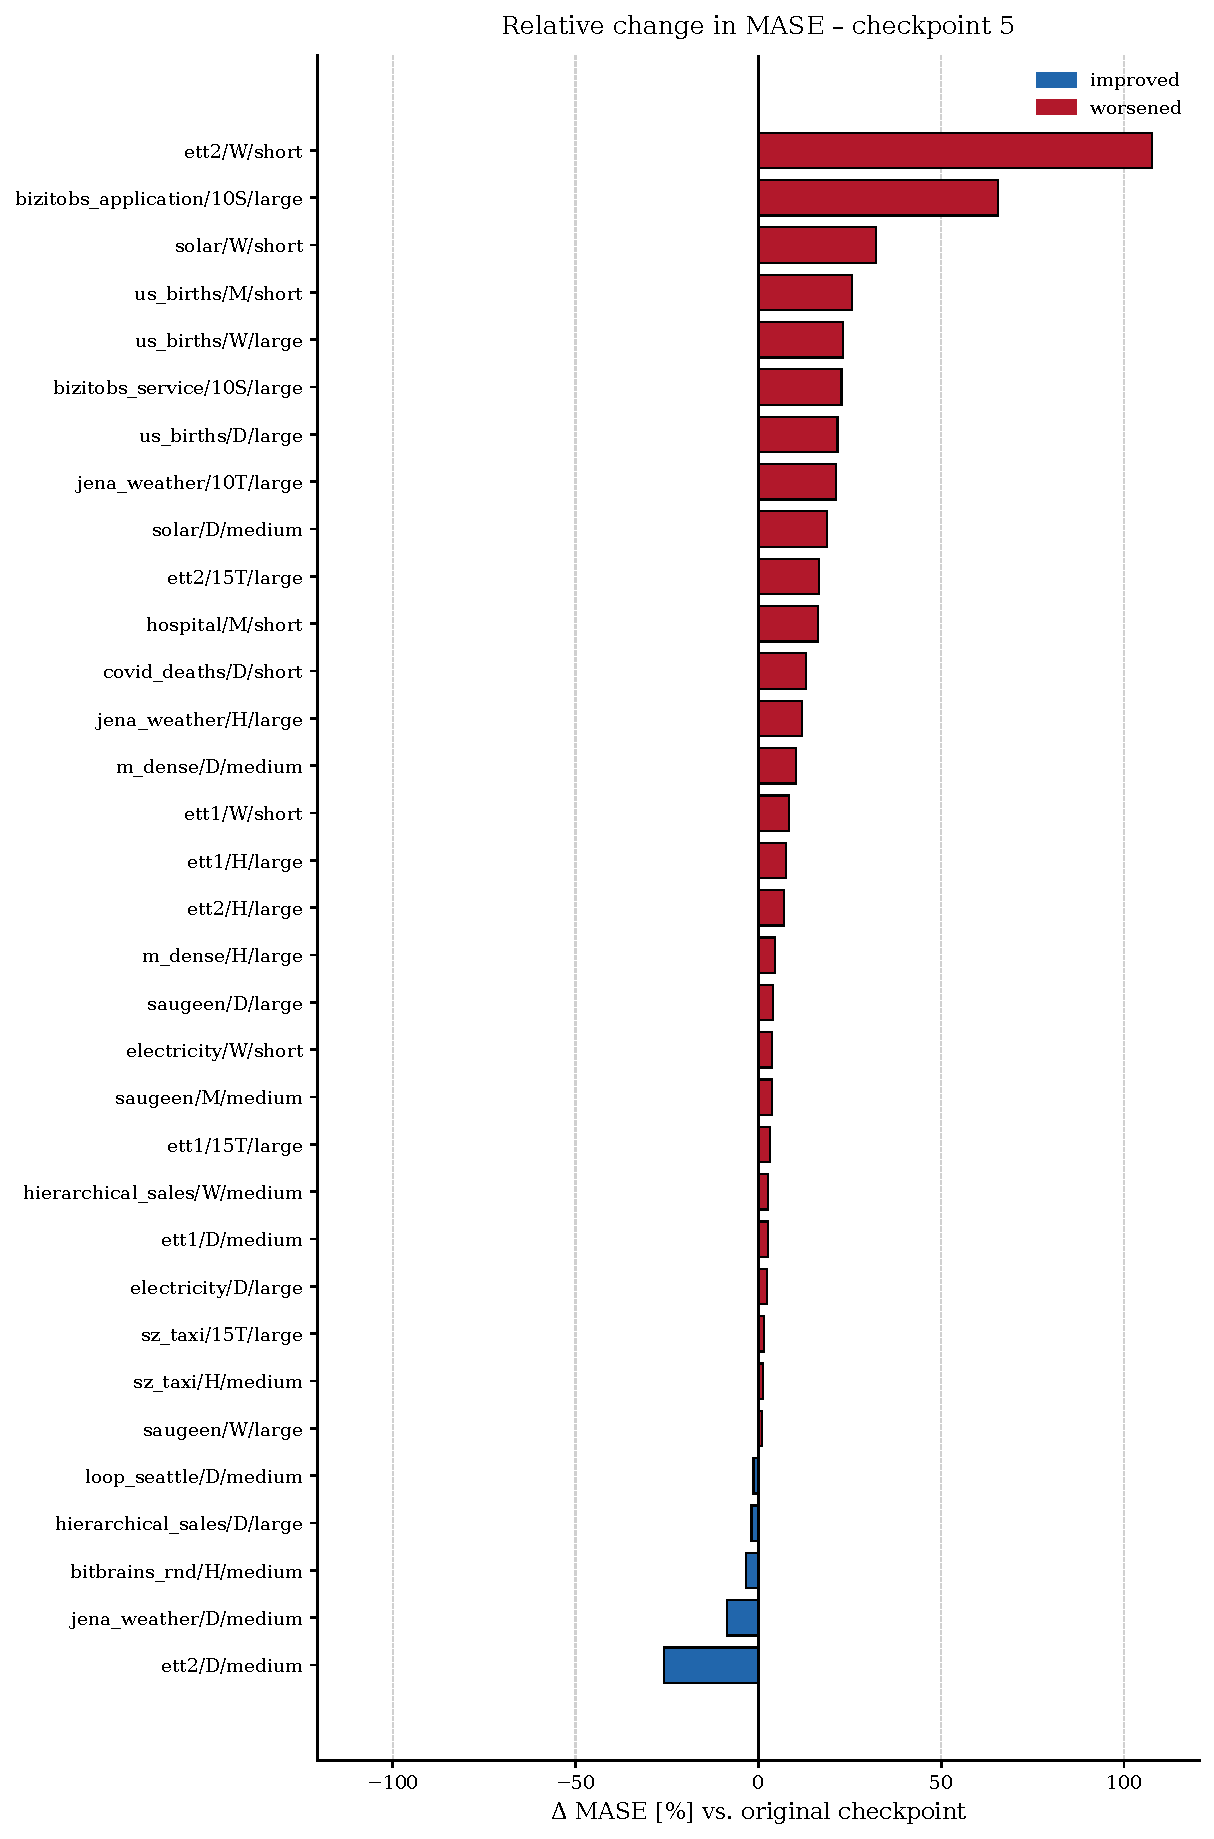
\includegraphics[width=\linewidth]{pictures/prior/mase_ckpt_5_delta_plot.pdf}
        \caption{Delta of checkpoint 5}
        \label{fig:mase_ckpt_5_delta_plot}
    \end{subfigure}

    \caption{Comparison of mean and checkpoint-wise delta plots. Lower is better. }
    \label{fig:combined_delta_plots}
\end{figure}
As shown in Figure~\ref{fig:mase_mean_delta_plot}, the mean performance across all five checkpoints improves on only three datasets, while it deteriorates on the remaining ones.
However, when analyzing individual checkpoints, differences become apparent. Checkpoints 1 and 2 both improve performance on 9 out of 18 datasets, whereas checkpoints 3, 4, and 5 show improvements on only a small number of datasets.
Furthermore, the improvements vary noticeably across datasets. While some datasets show noticeable gains, others exhibit negligible changes or even significant performance degradation.

The results also indicate that the effect of continued pretraining is highly dataset-dependent.
For example, datasets such as \textit{ett2/D} show consistent improvements across multiple checkpoints, whereas others such as \textit{ett2/W} and \textit{solar/W} do not benefit from continued pretraining at all.
Notably, datasets with shorter context lengths, such as \textit{solar/W} (context length 52), appear to be particularly challenging.

\iffalse
As one can see in plot~\ref{fig:mase_mean_delta_plot}, the mean performance over a selected set of datasets improved only on three datasets but worsened on all others.
This is a result of averaging the MASE scores over all 5 selected checkpoints.
Checkpoints 1 and 2 in the selection improved better as they both improved on 9 datasets.
But some of this performance is so minimal that one can say it stayed the same.
Another thing that is interesting to observe is that continued pretraining does not work on some datasets at all.
These are, for example, ett2/W and solar/W.
Both of which are datasets that have a short context length (103 and 52)
\fi
% Erster und zweiter Checkpoint performt auf mehreren Datensets gut aber hat auf manchen auch sehr starke Verluste

% Andere 3 Checkpoints sind viel schlechter zt -> nur auf 2 Datensets maximal

% Es gibt Datensets, auf denen der Prior generell gut ist, und manche, auf denen er überhaupt nicht gut ist.


\begin{table}[H]
\centering
\resizebox{0.8\textwidth}{!}{
\begin{tabular}{lcccccccccccccc}
\hline
Ckpt & Time & LR & Batch & L2-SP & WD & Time & Init & Best & Last & Steps & Best & ES & Time/ & Util \\
     & Limit &     &       &       &     & Spent & Val & Val & Val &       & Step &    & Step  &      \\
\hline
ckpt\_1 & 3600 & 0.0005 & 8 & 0.0001 & 0.0 & 3578.13 & 0.3624 & 0.2636 & 0.3315 & 115 & 79  & Time     & 31.11 & 35.33 \\
ckpt\_2 & 3600 & 0.0005 & 8 & 0.0    & 0.0 & 3585.33 & 0.3624 & 0.2762 & 0.2899 & 114 & 89  & Time     & 31.45 & 33.89 \\
ckpt\_3 & 3600 & 0.0005 & 2 & 0.0001 & 0.0 & 3603.73 & 0.3624 & 0.2812 & 0.2905 & 427 & 289 & Time     & 8.44  & 14.52 \\
ckpt\_4 & 3600 & 0.0005 & 2 & 0.0015 & 0.0 & 3336.01 & 0.3624 & 0.2861 & 0.5537 & 400 & 189 & AdaptES  & 8.34  & 14.19 \\
ckpt\_5 & 3600 & 0.0005 & 4 & 0.0    & 0.0 & 3669.10 & 0.3624 & 0.2912 & 0.2912 & 250 & 249 & Time     & 14.68 & 20.05 \\
\hline
\end{tabular}
}
\caption{Training results across checkpoints.}
\label{tab:training_results}
\end{table}
Table~\ref{tab:training_results} summarizes the hyperparameter configurations and training results of the top five checkpoints.
All selected checkpoints were trained with a learning rate of 0.0005. Configurations using smaller learning rates (e.g., 0.00005 and 0.000005) resulted in consistently worse validation performance and were therefore not included among the top checkpoints.
Regarding batch size, the top-performing checkpoints (ckpt\_1 and ckpt\_2) were trained with a batch size of 8, while other checkpoints used batch sizes of 2 or 4.
Additionally, a difference in the number of training steps can be observed. Checkpoints 1 and 2 performed significantly fewer steps (approximately 115) compared to checkpoints 3–5, which executed up to 427 steps.

Another notable observation is that four out of five checkpoints stopped training due to the time limit rather than early stopping based on validation performance.
Only checkpoint 4 terminated due to early stopping (AdaptiveES), indicating that most runs were constrained by the predefined training time.

\iffalse
By looking at table~\ref{tab:training_results}, one can see that all five checkpoints were trained with a learning rate of 0.0005.
The other checkpoints that yielded worse validation loss were mostly trained with learning rates smaller than this (0.00005, 0.000005), as shown in~\ref{TODO}.

Another interesting aspect is the step amount.
As mentioned above, the first two checkpoints performed significantly better on multiple datasets than the last three.
These two checkpoints also happen to have many fewer steps than the last three.
While ckpt\_1 and ckpt\_2 have a total of 115 and 114 steps, ckpt\_3, ckpt\_4, and ckpt\_5 have at least double the number of steps.
A cause for this could possibly be that the batch size of checkpoints 1 and 2 is both 8, thus needing more data to generate (that is why they also need double the time)
But they also perform significantly better.
Batch size 8 seems to be superior.
Another thing that comes to mind is that 4 of 5 checkpoints stopped training due to the time limit, not because the validation loss did not improve.
This is another important factor since ckpt\_1 and ckpt\_2 both needed much more time per step and could possibly improve even more
\fi
% hier so wie Single-Finetuning-Graphen und so zeigen weil ist ja nicht viel anders und wir haben auch viele Datensets

% Scatterplot mit x original und y prior MASE-Wert und diagonale
% prozentual Plot der Verbesserung zeigen Balkendiagramm

% Performance von 1. Checkpoint alleine auch zeigen
% vielleicht auch Performance von allen anderen Checkpoints auch zeigen



% Viele Trainingsläufe haben nicht aufgehört weil Patience auslief sondern weil Zeit vorbei war
% beste HP Konfig auf jeden Fall mit 0.0005 lr
\section{Discussion}
In our expose we defined the following question for this section:
"Can we continue pre-training TabPFN for time series with a prior that generates time series data (and does it improve performance)?"
This question can be answered positively, although the results indicate limitations, and the approach does not perform as well as initially expected.

A prior for time series should be able to generalize across different time series characteristics and yield better, more consistent results.
However, in our case with the prior we used from \citep{dooley2023forecastpfn}, this is not the case, as the effect we observed is very heterogeneous and, on average, only leads to better results on a small number of datasets.
A worsening of TabPFNs' performance is an effect we are looking at.
In the results section and what can be seen in <fig ref>, we can conclude that TabPFN only improved on 4 datasets but deteriorated on 20 other datasets.
These results alone are not sufficient to conclude that training with these prior results results in improved performance.

An especially interesting aspect was the behavior of the five checkpoints we selected based on their validation loss during training.
Checkpoints 1 and 2 perform significantly better than the other three checkpoints.
TabPFN improved performance on 12 and 11 datasets using these two checkpoints.
This suggests that these two checkpoints have different characteristics during training that allowed them to better adapt to the time series training data.

If we take a look at the hyperparameters that were used for the five checkpoints, we can observe that both of the top checkpoints used a batch size of 8, contrary to the other three, which used 2 and 4.
Empirically, this lets us assert that a batch size of 8 with a learning rate of 0.0005 is a good hyperparameter configuration for continued pretraining.

The training duration, measured by the number of steps/epochs we trained TabPFN on, also helps us conclude on another important factor for continued pretraining.
Both checkpoints 1 and 2 were trained for a total of 114/115 steps and reached their best performance at steps 79 and 89.
The other three checkpoints trained significantly longer, with up to 400 steps, while reaching their best state at step 189.
The consistently stronger performance of the early checkpoints suggests that moderate continued pretraining may be beneficial, while prolonged training may instead be harmful.
\newline
All checkpoints also ended due to the time limit of at most 40 minutes, instead of early stopping due to no improvements regarding the validation loss.
On the one hand, the reaching of this time limit comes from the data generation that is done dynamically while training.
On the other hand, this suggests that, since all runs were terminated due to the time limit rather than exhausted patience, the current results may not yet fully reflect the method’s potential.

For some datasets, it can be observed that the performance of all checkpoints consistently deteriorates, whereas for others it consistently improves.
This suggests that, while evaluation can also be different between checkpoints, it is also dataset-dependent.
Datasets that only experience a worsening mostly show difficult characteristics, such as noisy or intermittent time series, that even initially make it hard for TabPFN to forecast.

Finally, we can conclude that continued pretraining with a time-series-generating prior shows promising results, but it is not as general as one might think.
Our work here is limited only to the prior constructed by \citep{dooley2023forecastpfn}.
Future work should also focus on other time-series priors, as the general concept of further training a model with artificial time-series data yielded acceptable results.
% 1. High-level conclusion
% 2. Overall prior effect (heterogeneous)
% 3. Checkpoint behavior (early vs late)
% 4. Hyperparameter sensitivity
% 5. Training constraints (time limit)
% 6. Dataset dependency (datasets that don't perform well don't have the specific time series characteristic)

% prior effect nicht so wie gewünscht
% eher selektiv als globale Verbesserung
% heterogene statt homogene Effekte

% dataset dependent

% Checkpoints unterschiedlich -> frühe Checkpoints waren hier besser was darauf hindeuten kann dass mehr Training nicht gleich besser ist
% effizientes Training besser

% sehr hyperparameter empfindlich
% zu große Batch Sizes führen zu nichts und brauchen zu lange
% zu kleine Learning Rate zu konservativ

% Die konsistent besseren Ergebnisse der frühen Checkpoints deuten darauf hin, dass moderates Continued Pretraining nützlich sein kann, während längeres Training eher schadet.
% „Da alle Runs durch das Zeitlimit und nicht durch ausgeschöpfte Patience beendet wurden, ist es plausibel, dass die derzeitigen Ergebnisse das Potenzial der Methode noch nicht vollständig abbilden.“

% für manche Datensets stellt der Prior die Verteilung besser dar als für andere


% Conclusion bzw eher an den Anfang und Frage beantworten
% prior führt nicht zu einer klaren Verbesserung auf allen Datensets sondern hat eine Art Trade-off
% auf manchen Datensets wird es viel besser und auf manchen gar nicht
% hängt auch oft von der zugrunde liegenden Veteilung ab die ein Datenset hat und die des Prior